\section{End-to-end System}

By an \textit{end-to-end} system, we refer to a question answering system where the individual parts of the system are not fine-tuned or modeled for specific sub-tasks, and a single model is trained to take the question as well as passages/documents as inputs and produce the answer as an output, without any explicit indication of the question/answer type. To train such a system, we make enhancements to the existing state-of-the-art end-to-end QA systems, which we describe in the subsequent sections.

\subsection{Dynamic Co-Attention Networks}

For span prediction, we implement a modified variant of the Dynamic Co-Attention Network (DCN) architecture. This architecture is composed of an encoder segment and a decoder segment. The encoder segment first encodes the question and document word vectors with a bidirectional GRU. It then computes an attention both from the question text to the passage and from the passage to the question text to identify the most relevant information for each word in the passage-question pair. The computed attention over the words are fused to add contextual information to each word vector in the passage. In particular, the fusion process finds the soft dot attention from the question to the passage, from the passage to the question, and from the passage to the fused question-passage vectors:

\begin{align*}
D, Q: &\text{ The passage and question matrices, where each row is a word vector} \\
L: &\text{ Dot affinity matrix} = D Q^T \\
C^Q: &\text{ Fused question-passage attention matrix} = \softmax(L) Q \\
C^D: &\text{ Fused passage-question attention matrix} = \softmax(L^T) D \\
{C^D}': &\text{ Fused passage-(question-passage) co-attention matrix} = \softmax(L) C^Q \\
\end{align*}

This process is repeated with $C^D$ replacing $D$ and $C^Q$ replacing $Q$ to produce a new set of matrices $C^{C^D}$, $C^{C^Q}$ and $C^{C^D \prime}$. The concatenation $[D, C^D, C^{D \prime}, C^{C^D}, C^{C^D \prime}]$ is finally passed to a second bidirectional GRU to produce a semantically rich and meaningful representations for each of word in the passage.

The decoder uses a GRU to iterate over the encoded passage vectors, predicting and iteratively improving its estimate of the start and end markers of the answer span:

\begin{align*}
u_t: &\text{ The encoding of the t\textsuperscript{th} word in the passage} \\
h_t: &\text{ The GRU hidden state at iteration t} = GRU(h_{t - 1}, s_t, e_t) \\
\text{HMN}: &\text{ Highway maxout network} \\
s_t: &\text{ The probability vector for the location of the start marker at iteration t} = \text{HMN}(h_{t - 1}, s_{t - 1}, e_{t - 1}) \\
s_t' &\text{ A one-hot vector corresponding to the location of } s_t \text{ with highest probability}. \\
e_t: &\text{ The probability vector for the location of the start marker at iteration t} = \text{HMN}(h_{t - 1}, s_t', e_{t - 1})\\
\end{align*}

This iterative procedure enables the model to recover from initial local maxima corresponding to incorrect answers. This alleviates one of the major issues with question answering systems where they fail to make iterative refinements to the answer based on the context they learn. The traditional systems also fail to learn transitive relations for example they fail to identify the subjects which certain pronouns correspond to due to their single pass answer generation nature. On the other hand, the dynamic pointing encoder can resolve such relationships as it scans through the encoded passage vectors to predict the start and end markers.\\

\subsubsection{Network Architecture}
The encoder architecture is presented in Figure \ref{im:enc} and the Decoder architecture for DCN is presented in Figure \ref{im:dec}.

\begin{figure}[h]
    \centering
    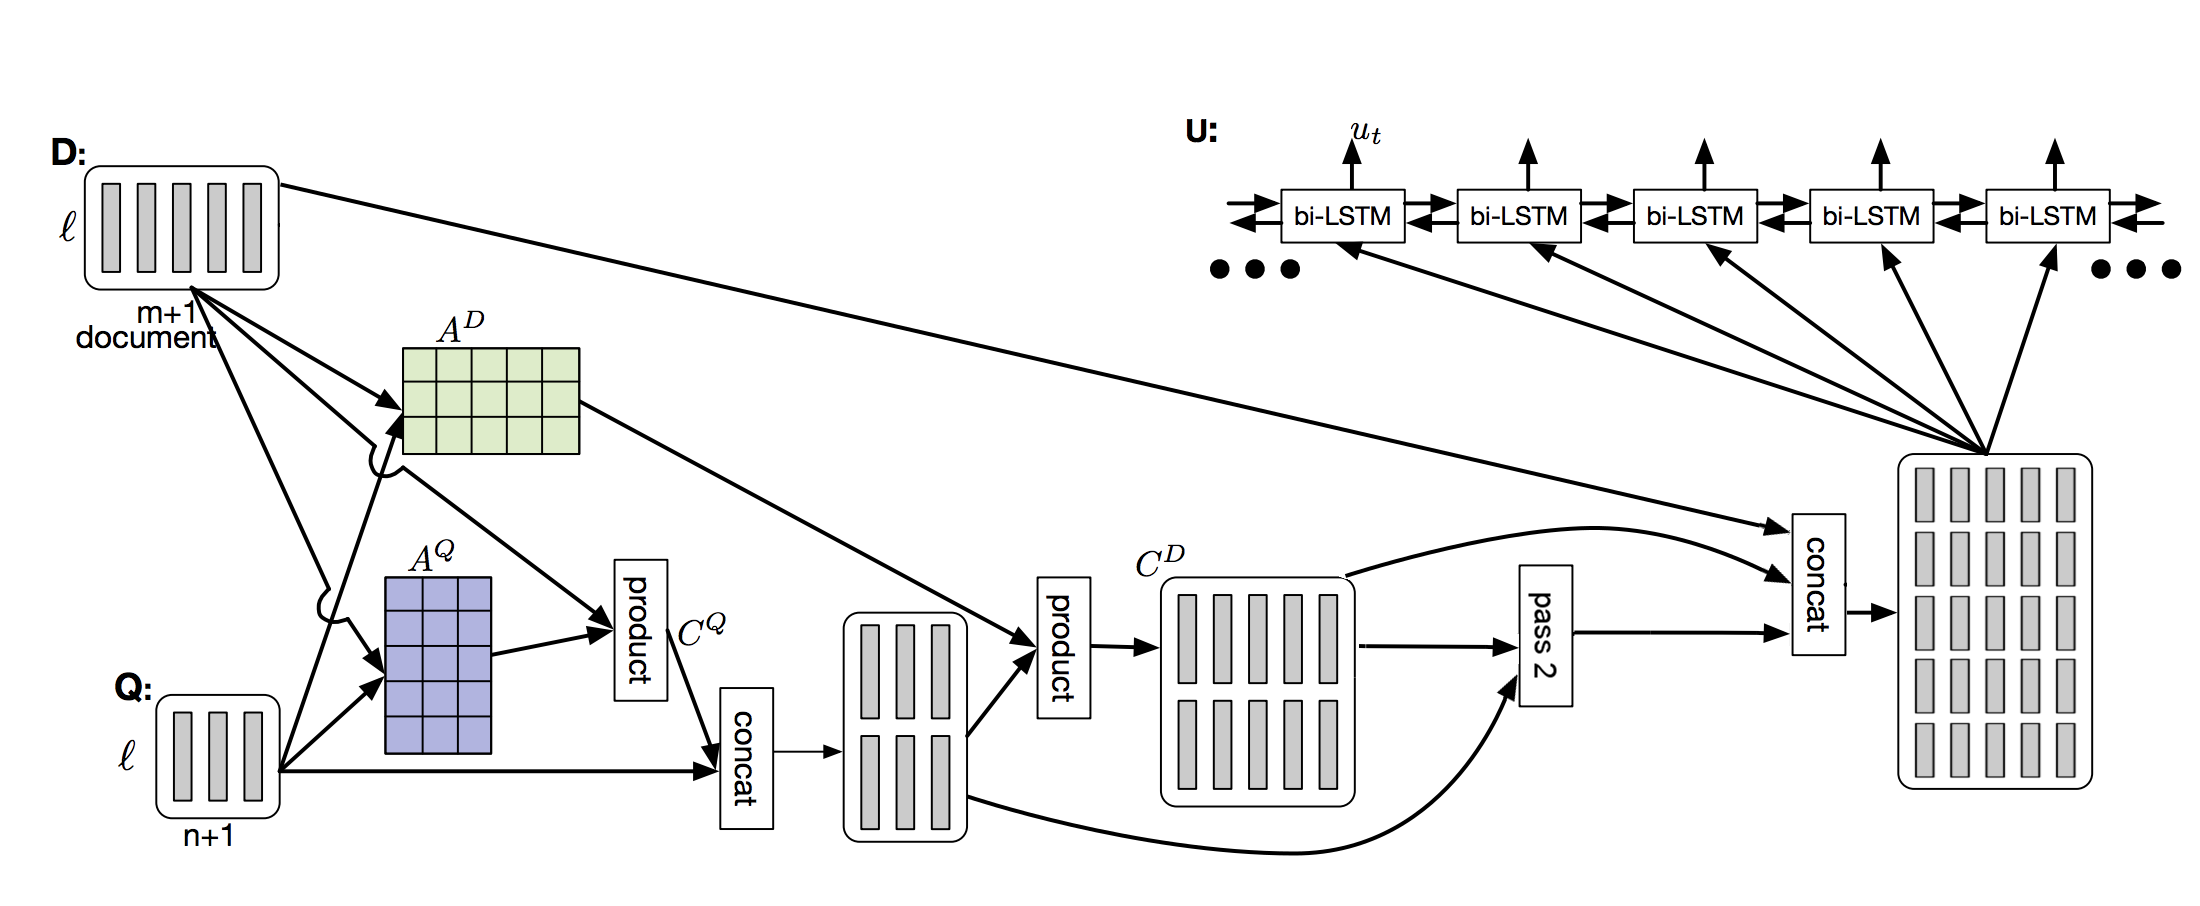
\includegraphics[width=0.9\textwidth]{images/coattn_encoder.png}
    \caption{The DCN Co-attention Encoder}
    \label{im:enc}
\end{figure}

\begin{figure*}[h]
    \centering
    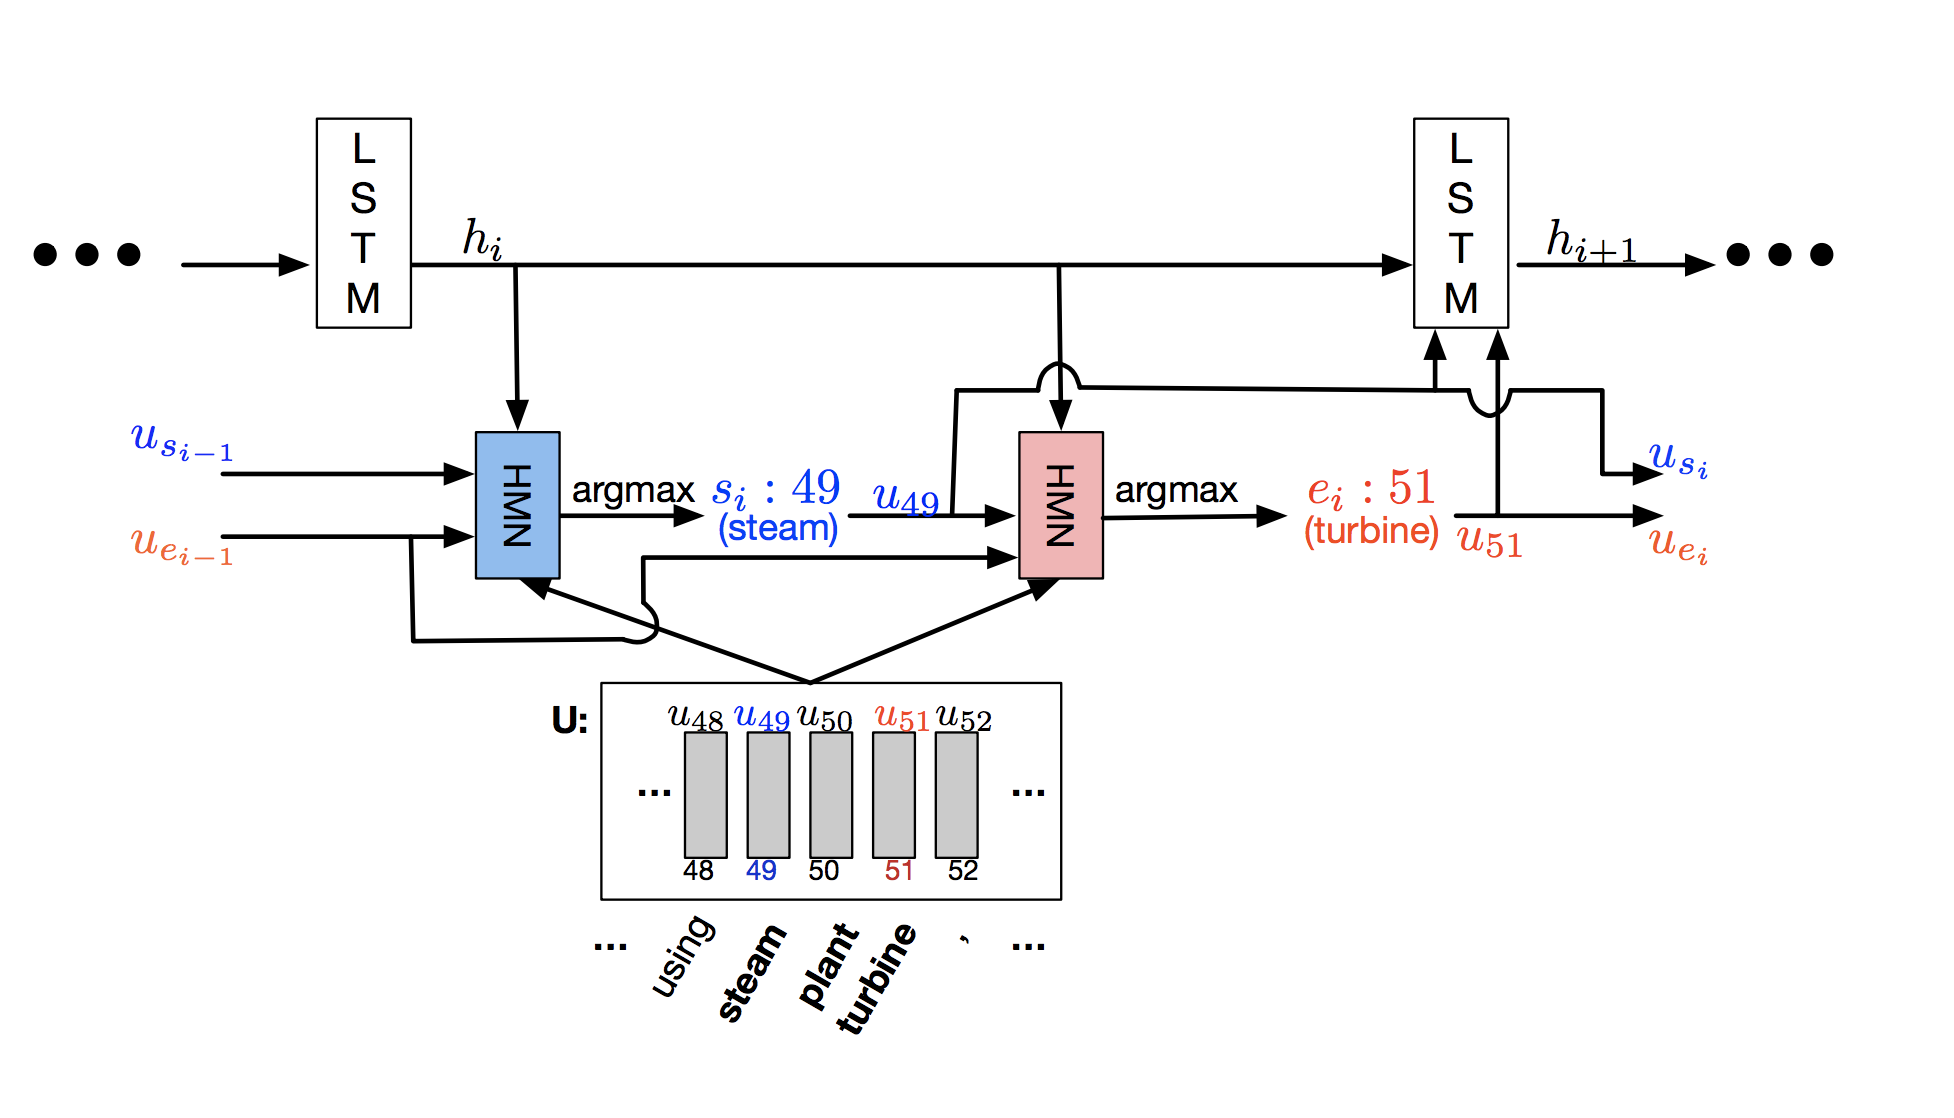
\includegraphics[width=0.85\textwidth]{images/decoder.png}
    \caption{The Dynamic Decoder Network}
    \label{im:dec}
\end{figure*}

\subsubsection{Experiments}

We first compute the GLoVe and CoVe word vectors for each word in the training and development data of the Stanford Question Answering Dataset (SQuAD) dataset, replacing all out of dictionary words with the zero vector. Then the network is trained with the Adam optimizer and the cross entropy loss for 40 epochs on a K80 GPU. A three-layer GRU network is used in the decoder network for all experiments, but we adjust the number of hidden units for the GRU networks that exist in the architecture. Experiments with 30, 100 and 200 hidden units per GRU are performed. An annealed learning rate initialized at 0.002 and a weight decay of 0.0001 is used during the training process. Gradient clipping is employed to prevent large gradients from destabilizing the training process, and early stopping is employed to stop training once overfitting is detected.

\subsection{Results on SQuAD}
The results on SQuAD with all the different variety of approaches we tried are presented in Table \ref{im:squad_res}. We present the results in a step by step fashion, showing how each of our modifications improves the results. We also note that we train our model for just 20 epochs compared to over 200 epochs used by the original model. Our best performing model qualifies to be ranked on the official SQuAD leader board.

\begin{figure*}[h]
    \centering
    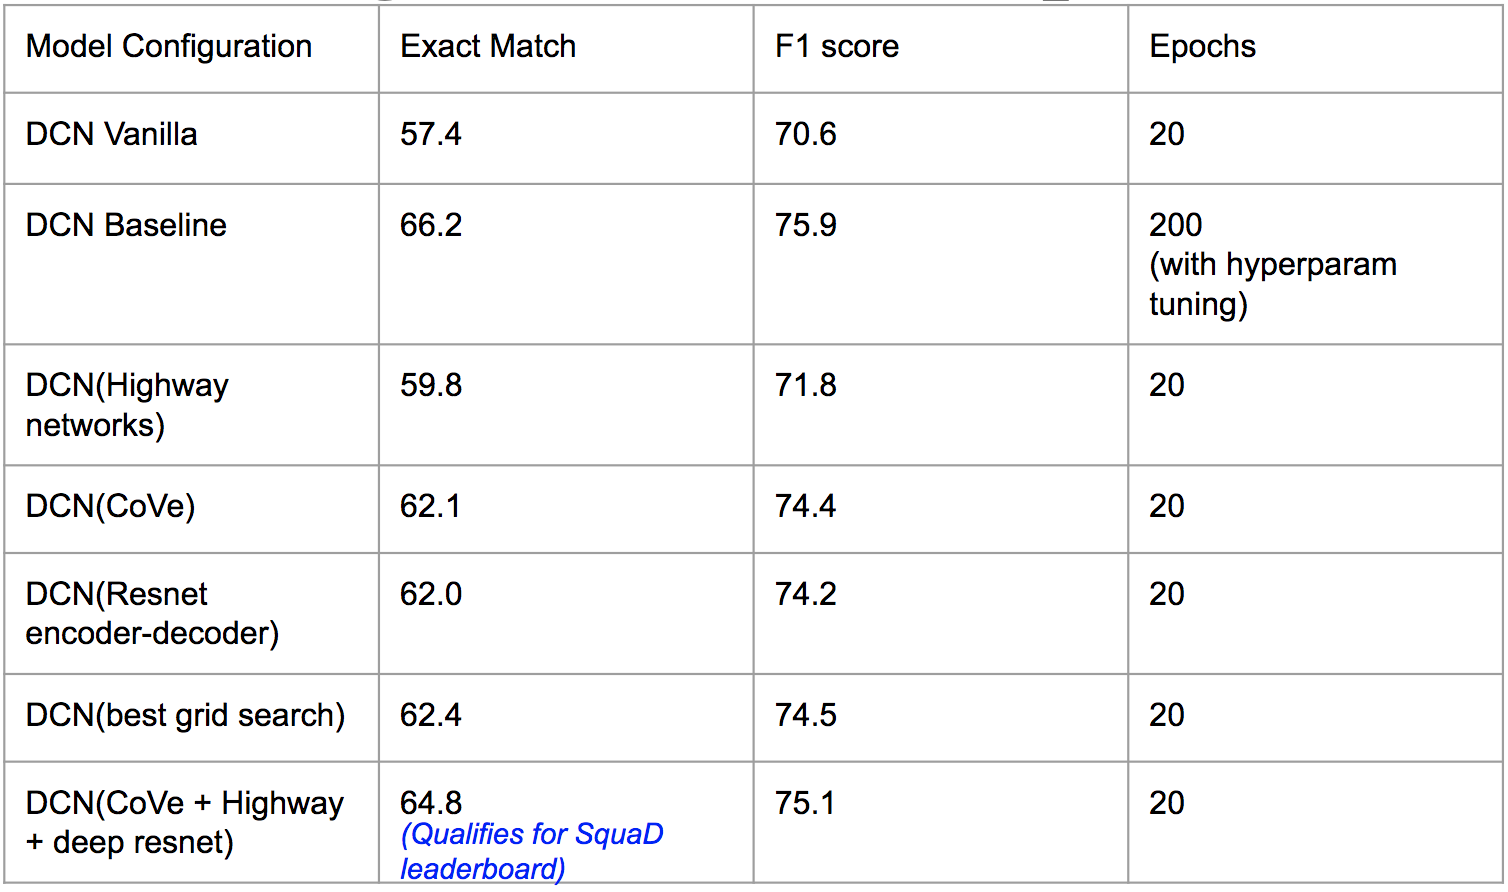
\includegraphics[width=0.85\textwidth]{images/res_squad.png}
    \caption{Results on the SQuAD dataset}
    \label{im:squad_res}
\end{figure*}

\begin{figure*}[h]
    \centering
    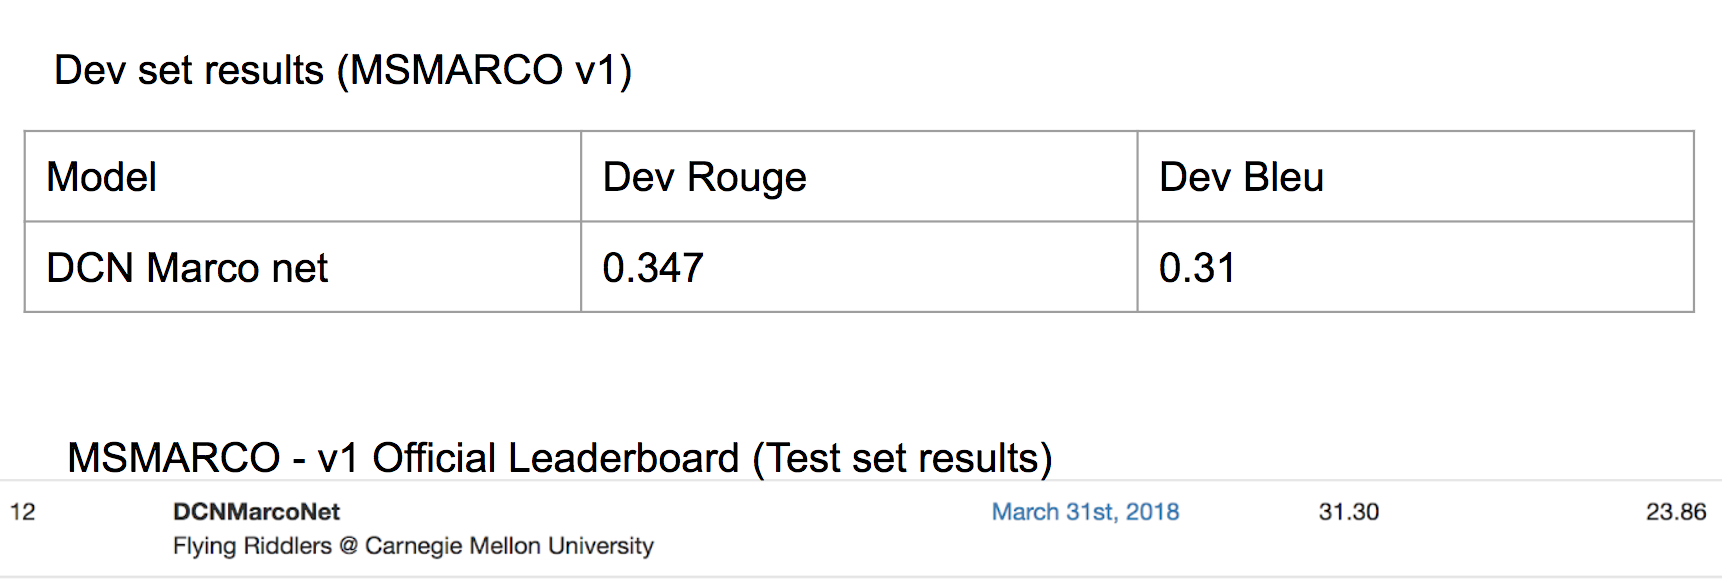
\includegraphics[width=0.85\textwidth]{images/res_marco.png}
    \caption{Results on the MSMarco v1 dataset}
    \label{im:res_marco}
\end{figure*}


An informal test is also performed with a small number of test cases not found in the data set. We find that the trained network has the capacity to answer these questions accurately as well. One out-of-dataset example is shown below:

\begin{table}
\begin{tabular}{|c|p{0.75\textwidth}|}
    \hline
    Document & The de Broglie–Bohm theory, also known as the pilot wave theory, Bohmian mechanics, Bohm's interpretation, and the causal interpretation, is an interpretation of quantum theory. In addition to a wavefunction on the space of all possible configurations, it also postulates an actual [...] The theory is named after Louis de Broglie (1892–1987) and David Bohm (1917–1992). \\
    \hline
    Question & After whom is pilot wave theory named after? \\
    \hline
    Predicted answer & Louis de Broglie \\
    \hline
\end{tabular}
\end{table}

This example demonstrates the ability of the network to resolve indirect relationships in the text, such as the chain connecting the phrase ``The theory [is named after]'' to its referent ``The de Broglie–Bohm theory'' to its alternative name ``the pilot wave theory''.

\subsection{Free Form Answer Generation}

Free Form answer generation is a relatively unexplored problem with little existing literature. Trying to solve this problem directly is a fairly hard task and would require an extremely complex network architecture which can not just look at huge text sources to detect the most relevant parts, but also compose a human like answer. This is too hard for most networks to achieve. To reduce the complexity of the problem being dealt by a single network, we use the spans predicted by our Dynamic Co-Attention Network as input to the Free Form answer generator network. This makes the network more powerful by giving it more information about the content of the expected answer and it now has to use this content information to compose an answer. \\

Natural Language generation is known to be one of the hardest problems on the NLP community due to the inability of modern day architectures to model long term context and generate syntactic and semantically coherent sentences. One of the primary issues we notice with such architecture is the ineffectiveness of the loss functions typically used in the seq2seq prediction networks typically used for this task. The seq2seq networks are usually based on LSTM encoder - decoder style architectures and typically penalize the generator using a cross entropy loss between the predicted and expected output word. Such work level loss metrics fail to capture global sentence level dynamics and completely miss out on enforcing syntactic and semantic coherence. We propose a novel loss metric here which we feel would be greatly useful in dealing with such issues.\\

First we introduce our generator network architecture. The architecture we propose is shown in Figure \ref{im:im_gen}.
\begin{figure*}[h]
    \centering
    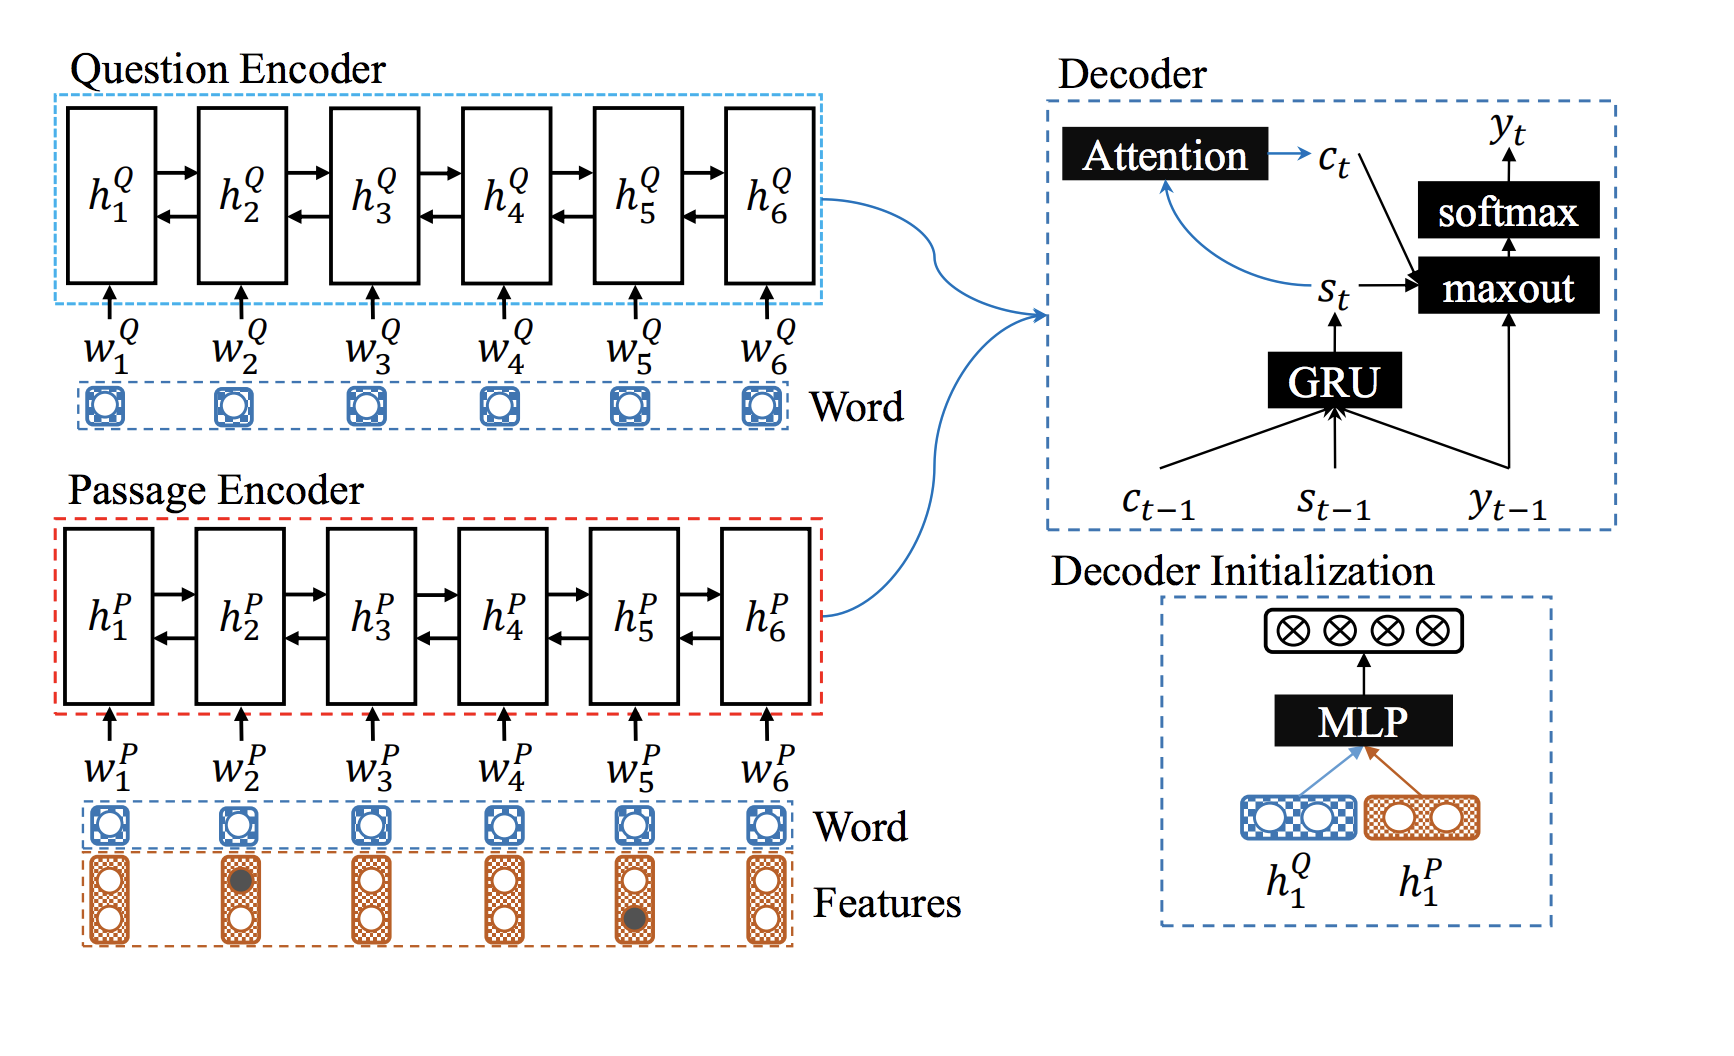
\includegraphics[width=0.85\textwidth]{images/ans_net.png}
    \caption{The Answer generator Network}
    \label{im:im_gen}
\end{figure*}

The network consists of a question encoder network, a paragraph encoder network and an attention based decoder network.\\
The question and passage encoder are Bidirectional GRU's which take as input the question and passage word embeddings, one word at a time and generate the respective question and passage embedding. This is given by the equations:

\[ {h_t}^P = BiGRU({h_{t-1}}^P, [{e_t}^P, {f_t}^e, {f_t}^e]) \]

\[{h_t}^Q = BiGRU({h_{t-1}}^Q, {e_t}^Q) \]

here ${h_t}^P$ and ${h_t}^Q$ denote the passage and question encoder hidden state at time t, ${e_t}^P$ and ${e_t}^Q$ denote the word embedding of  passage and question word at time t, ${f_t}^e$, ${f_t}^s$ are binary bits which are 0 or 1 depending of if the $t^{th}$ word in the passage is the start or end of a span i.e.  ${f_t}^e = 1$ if the $t^{th}$ word is the end of a span and 0 otherwise. Similarly ${f_t}^s = 1$ if the $t^{th}$ word is the start of the answer span and 0 otherwise.\\
The decoder is also a GRU which has a non linear combination of the question and passage encoding as its initial state denoted by:
\[ d_0 = tanh(W_d[{h_1}^P, {h_1}^Q] + b) \]
The rest of the decoder can be represented as:
\[d_t = GRU(w_{t-1}, {c^P}_{t-1}, {c^Q}_{t-1}, d_{t-1})\]
where $w_{t−1}$ is the word generated at the previous time step, $d_{t−1}$ is the previous decoder state and ${c^P}_{t-1}$ is the passage context vector which is learnt by computing the attention of the decoder state over the passage states. Similarly ${c^Q}_{t-1}$ is the context vector computed by taking the attention of the decoder state over the states of the question encoder. 

We experiment with two different types of attention mechanisms, which we call as the `additive attention mechanism' and the `dot attention mechanism'. \\
The additive attention mechanism is defined by the following equations.:\\
\[  {{s^P}_{t,j}} = {{v^P}_a}^Ttanh({W^P}_a(d_{t-1}) + {U_a}^P{h^P}_j )\]
\[{a^P}_{t,i} = softmax({{s^P}_{t,j}})\]
\[{c^P}_t = \sum_{i=1}^n {a^P}_{t,i} \cdot {h^P}_i\]

Similarly for question encodings:\\
\[  {{s^Q}_{t,j}} = {{v^Q}_a}^Ttanh({W^Q}_a(d_{t-1}) + {U_a}^Q{h^P}_j )\]
\[{a^Q}_{t,i} = softmax({{s^Q}_{t,j}})\]
\[{c^Q}_t = \sum_{i=1}^n {a^Q}_{t,i} \cdot {h^Q}_i\]

The dot attention on the other hand is defined by the equations:\\
\[  {{s^P}_{t,j}} = (d_{t-1})^T{h^P}_j \]
\[{a^P}_{t,i} = softmax({{s^P}_{t,j}})\]
\[{c^P}_t = \sum_{i=1}^n {a^P}_{t,i} \cdot {h^P}_i\]
Similarly for question encodings:\\
\[  {{s^P}_{t,j}} = (d_{t-1})^T{h^Q}_j \]
\[{a^P}_{t,i} = softmax({{s^P}_{t,j}})\]
\[{c^P}_t = \sum_{i=1}^n {a^P}_{t,i} \cdot {h^P}_i\]
These attention weighted question and passage encodings are fed to the decoder network.\\
To predict the next word we use the present decoder state, the question and passage context and the previous word and pass their combination through a Maxout layer, taking maxout over 2 successive units and then take a softmax over our vocabulary. This is represented by the equations:\\
\[r_t = W_rw_{t-1} + {U^P}_r{c^P}_t + {U^Q}_r{c^Q}_t + V_rd_t \]
\[m_t = [max{r_{t,2j-1}, r_{t,2j}}]^T \]
\[p(y_t|y_1, . . . , y_{t-1}) = softmax(W_o \cdot m_t) \]


\subsection{Results on MS MARCO}
We use our free form answer generation network on the MSMarco V1 dataset. The results for the same are listed in Table \ref{im:res_marco}. We note that we are listed as one of the highest ranked single model on the actual MSMarco leaderboard.

\subsection{Experiments and Results on BioASQ dataset}

We further extend our model to evaluate it on the BioASQ dataset. We use our DCN model to perform the QA task on the BioASQ dataset. Presently, we only work with factoid and list type of questions. The architecture is exactly the same as the DCN encoder. In place of the decoder we simply use the attention values over the passage to predict our answers. For both factoid and list type questions, the passage entities which attain attention more than a threshold are chosen as the correct answers. For the Factoid type answers, as the ranking of these entities also matters we return them in the order of decreasing attention weights. The results of this model evaluated on the BioASQ dataset after pre-training on the SQuAD dataset are presented in Table \ref{tab:bioasq_res}. Note that presently the model uses word2vec and Cove embeddings and hence several of the Biological entities are actually not a part of the vocabulary which may partially explain the poor performance of the DCN model on the BioASQ dataset.

\begin{table}
\centering
\begin{tabular}{|c|c|c|}
    \hline \hline
    Model & Factoid(MRR) & List(F1)\\
    \hline
    DCN MarcoNet& 0.11&0.07\\
    \hline \hline
\end{tabular}
    \caption{Results on the Bioasq dataset}
    \label{tab:bioasq_res}
\end{table}
